\draft Quantum Hall effect in a semiconductor.
Naturally the question is a lot more difficult due to its open-book nature.

\begin{parts}
	\part Heterostructure: by forming a sandwich of lower band gap between 2 p and n doped layers, a 2D electron gas is formed due to the confinement along layers, this can be further realised by populating only the lowest sub-band with low enough carrier density.
	
	Modulation doping:
	\begin{figure}[H]
		\centering
		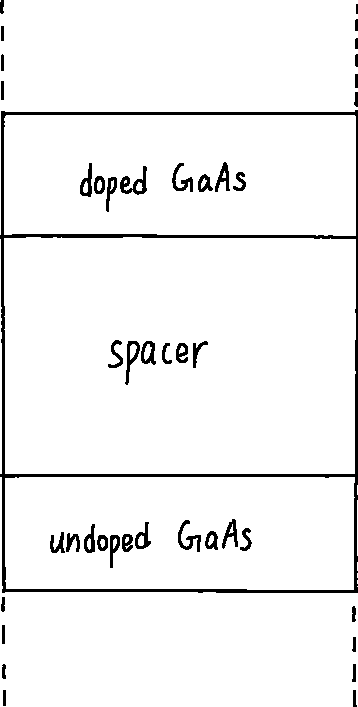
\includegraphics[width=.2\linewidth]{q2-modulation-doping}
	\end{figure}
	By repeatedly applying the layers shown above, we may modulate the doping of GaAs.
	This is important as the spacer separates the ionised donors from the electrons, thus reducing the scattering rate $\Rightarrow$ larger carrier mobilities.
	
	Sketch of conductivity $\sigma$ against temperature $T$ (silicon doping so n-type $\rightarrow$ no cusp due to change in dominant carrier):
	\begin{figure}[H]
		\centering
		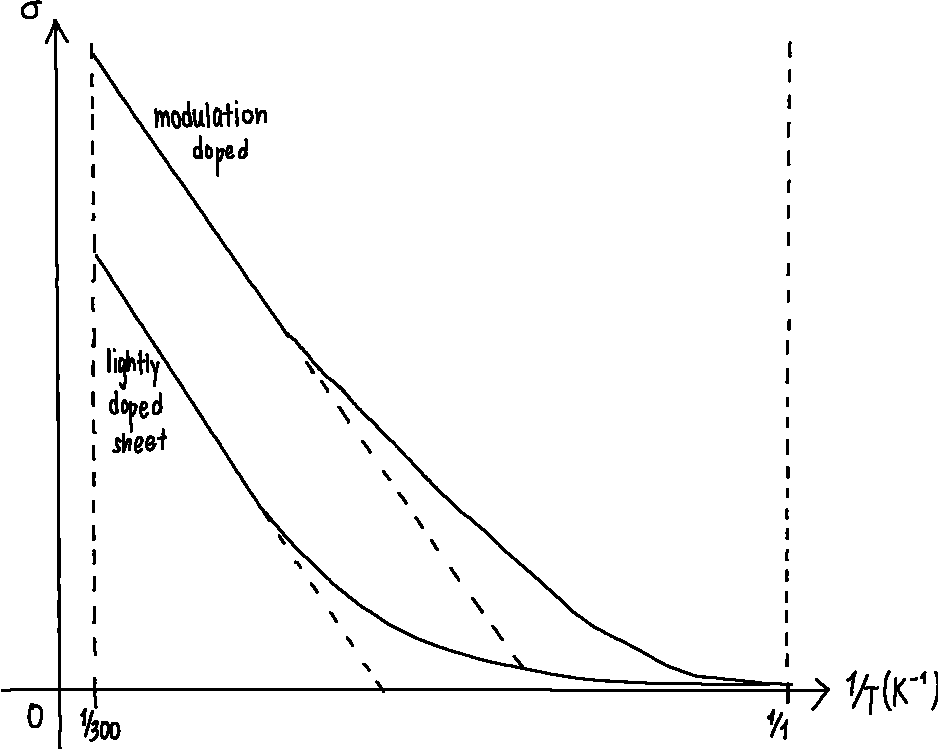
\includegraphics[width=.6\linewidth]{q2-conductivity}
	\end{figure}
	The temperature dependence arises from the freezing of thermally excited charge carriers.
	
	\part
	Sketch of an arbitrary energy surface:
	\begin{figure}[H]
		\centering
		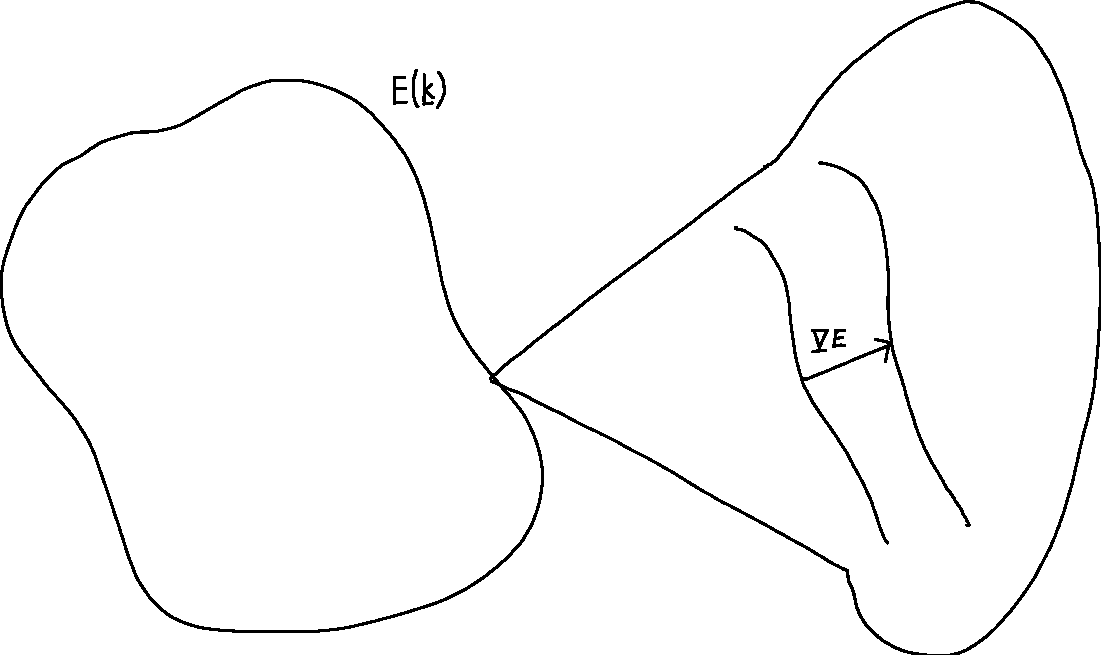
\includegraphics[width=.6\linewidth]{q2-grad-e}
	\end{figure}
	
	In 2D, where $g_e$ is the $\electron$ spin degeneracy:
	\begin{align*}
		g(k) \inftsml{k} &\rightarrow \frac{g_e}{\rbracket{2\pi}^2} \, \delta A \mtext{where $\rbracket{2\pi}^2$ comes from continuum approximation} \\
		\delta A &= \oint_{l} \inftsml{\mathbf{l}} \times \hat{\mathbf{n}} \mtext{where $\hat{\mathbf{n}} = \dfrac{\bm{\nabla}E}{\abs{\mathbf{\nabla}E}}$ is the normal unit vector to the iso-energy line} \\
		&= \oint_{l} \frac{\inftsml{l}}{\abs{\mathbf{\nabla}E}}
	\end{align*}
	
	For the conduction s-band, $E = \dfrac{\hbar^2 k^2}{2m^*} \Rightarrow \nabla E = \dfrac{\hbar^2 k}{m^*}$:
	\begin{align*}
		\delta A &= 2\pi k \cdot \frac{m^*}{\hbar^2 k} \\
		&= \frac{2\pi m^*}{\hbar^2} \\
		\Rightarrow g(E) &= \frac{2\pi g_e}{\rbracket{2\pi}^2 \hbar^2} m^* = \underbracket{\frac{g_e}{2\pi \hbar^2}}_{\alpha} m^*
	\end{align*}
	
	\part
	\begin{subparts}
		\subpart We know that \# of states per Landau level = \# of states between orbits at $B=0$:
		\begin{equation*}
			n_s = \frac{g_e \pi}{\rbracket{2\pi}^2} \rbracket{k_{n+1}^2 - k_n^2}
		\end{equation*}
		where $\frac{\hbar^2 k_n^2}{2m^*} = (n+1/2)\hbar\omega_c = (n+1/2) \hbar eB/m^* \Rightarrow k_n^2 = (n+1/2) 2eB/\hbar$:
		\begin{align*}
			\Rightarrow n_s &= \frac{g_e \pi}{\rbracket{2\pi}^2} \frac{2eB}{\hbar} \\
			&= g_e \frac{2\pi eB}{\hbar} \cdot \frac{1}{\rbracket{2\pi}^2} \\
			&= g_e \frac{eB}{h} \mtext{where the factor of $(2\pi)^2$ comes from continuum approximation}
		\end{align*}
		
		\subpart Total number of areal density:
		\begin{align*}
			n_s \nu &= N \\
			\frac{g_e eB}{h} &= \frac{N}{\nu} \\
			\Rightarrow \Delta\rbracket{\frac{1}{B}} &= \frac{g_e e}{hN} \\
			\Delta\rbracket{\frac{1}{B}} \cdot B &= \frac{1}{\nu} \\
			B &= \frac{1}{\nu \cdot \Delta\rbracket{1/B}}
		\end{align*}
		
		From the graph, we have:
		\begin{align*}
			\Delta\rbracket{\frac{1}{B}} &= \frac{1}{18} - \frac{1}{25} \\
			&= \num{0.0156}(\unit{\per\tesla})
		\end{align*}
		
		So for $\nu = 3$, $B = \SI{21.4}{\tesla}$.
		For $\nu = 4$, $B = \SI{16.1}{\tesla}$.
		For $\nu = 6$, $B = \SI{10.7}{\tesla}$.
		
		Sketch of $\rho_{xx}$ against $B$:
		\begin{figure}[H]
			\centering
			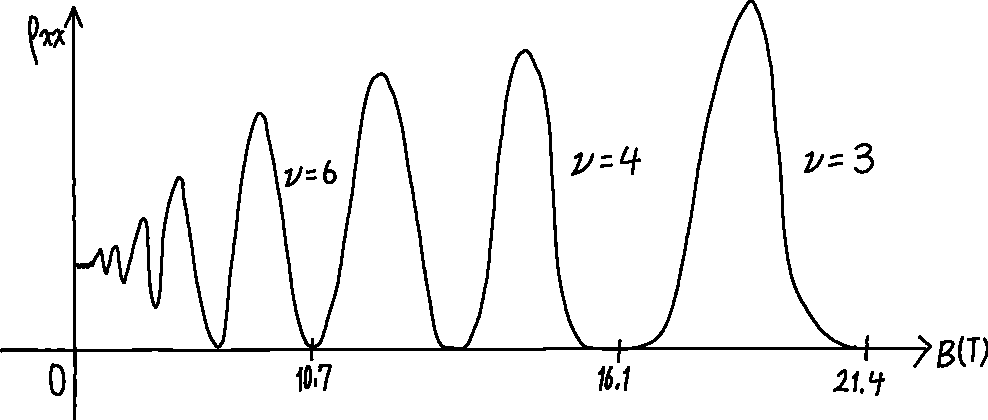
\includegraphics[width=.8\linewidth]{q2-resistivity}
		\end{figure}
		
		\newpage
		\subpart Sketch of $\mu$ against $B$:
		\begin{figure}[H]
			\centering
			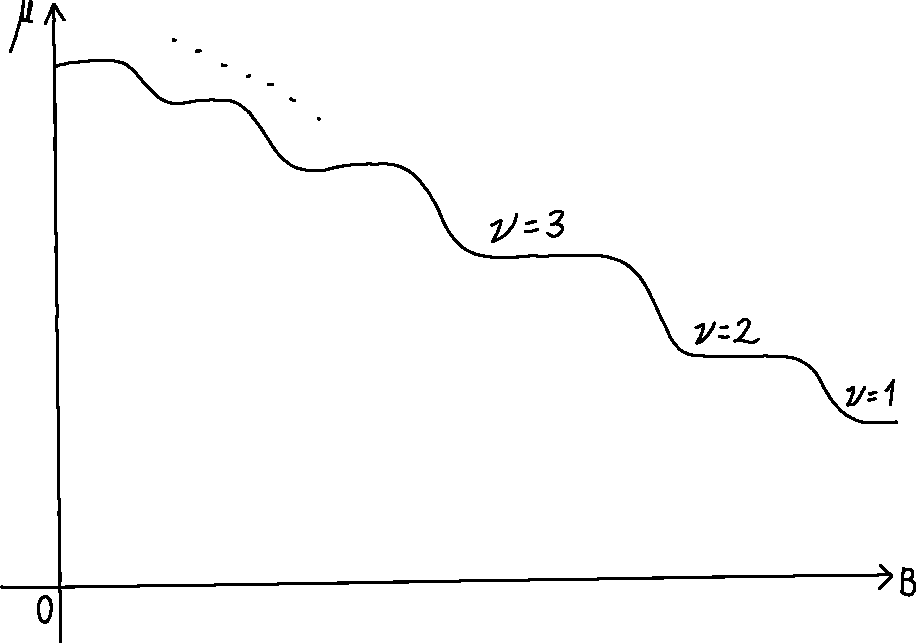
\includegraphics[width=.8\linewidth]{q2-chemical-potential}
		\end{figure}
		
		Ideally $\mu$ should be a series of Heaviside step function.
		However due to disorders, there are broadening near the boundaries of Landau levels, $\mu$ decreases as each Landau level is able to hold more states.
		
		\subpart From the graph, we have:
		\begin{align*}
			\Delta\rbracket{\frac{1}{B}} &= \frac{g_e e}{hN} = \SI{0.0156}{\per\tesla} \\
			\Rightarrow N &= \frac{g_e e}{h \Delta(1/B)} \\
			&= \SI{3.11e16}{\per\metre\squared} \\
			&= \SI{3.11e12}{\per\centi\metre\squared} = n_\textnormal{dopant} \mtext{assuming all charge carriers come from dopant}
		\end{align*}
	\end{subparts}
\end{parts}